\chapter{Sommaire (en Français)}
\label{chapter:sommaire}
\pagestyle{mainmatter}
\pagenumbering{arabic}

Comprendre le cerveau humain  est l'un des défis les plus importants du 21e siècle. Sans doute l'organe le plus complexe du corps humain, le cerveau est responsable  d’un large éventail de fonctions cognitives telles la reconnaissance visuelle, la compréhension du langage, la production de la parole, les interactions sociales et le contrôle exécutif. Les pathologies associées au cerveau demeurent, à ce jour, une problématique extrêmement complexe.  Actuellement, les interventions médicales pour les principales maladies infectieuses permettent aux individus de vivre jusqu'à l’âge de 80 et même  90 ans. Malgré les avancées de la médecine, nous n’arrivons pas à cibler efficacement les mécanismes  qui engendrent ou qui contribuent à la progression des pathologies mentales, telles le Parkinson, la démence d’Alzheimer, la schizophrénie  et l’épilepsie, pour n'en nommer que quelques-unes. Ceci a de graves conséquences sur la société vieillissante, par exemple une personne  dans la quarantaine a 50\% de risque de développer la maladie d'Alzheimer ~\citep{alzheimer20162016}.

Néanmoins, notre compréhension actuelle du cerveau est le résultat de décennies d'efforts concertés dans de multiples disciplines allant de la biologie moléculaire, à la génétique et la physiologie, en passant par les neurosciences cognitives et comportementales, la statistique, l'informatique et la science des données. Un sous-domaine en expansion est l'imagerie cérébrale, également connue sous le nom de neuroimagerie. L'imagerie cérébrale fait référence à un ensemble de technologies où l'on mesure l’activité  instantanée du cerveau. Ces mesures peuvent être statiques, comme dans le cas des images anatomiques issues de l'imagerie par résonance magnétique (IRM), ou dynamique, comme dans le cas de l'imagerie par résonance magnétique fonctionnelle (IRMf). L’objectif à long-terme serait d’utiliser ces techniques  dans les hôpitaux pour aider au niveau du diagnostic et dans les chirurgies, dans les interfaces cerveau-machine (BCI) et dans la recherche en neurosciences. Cette thèse sera dédiée à  la mesure des courants électriques et/ou du champ magnétique du cerveau par l’entremise de l'électroencéphalographie (EEG), de la magnétoencéphalographie et les potentiels de champ local (LFP). Ces méthodes ont la propriété de posséder une résolution temporelle élevée,ce qui est particulièrement utile pour extraire la dynamique temporelle des signaux du cerveau.

Dans cette thèse, j’élabore sur l’optimisation des analyses  de données publiques en  neuroimagerie , et ce, au moyen des logiciels libres. À cet effet, j'ai participé à une collaboration internationale pour créer une norme sur les analyses en MEG pour la structure de données d'imagerie cérébrale (BIDS)~\citep{niso2018meg}. J'ai écrit le validateur qui a aidé à créer les exemples d'ensembles de données compatibles MEG-BIDS. En tant que collaborateur de MNE~\citep{gramfort2013meg}, j'ai dirigé la rédaction d'un tutoriel qui permet d’analyser à nouveau un ensemble de données, nommé Faces~\citep{wakeman2015multi}, pour une reproduire les résultats préalablement retrouvés.Dans le contexte du mouvement de reproductibilité et de partage des données, nous avons commencé à automatiser nos séquences d’étapes d’analyses (pipelines), ce qui nous a amené à développer un algorithme entièrement automatisé pour le rejet et la réparation des artefacts en EEG/MEG~\citep{jas2016automated, jas2017autoreject}. Enfin, nous avons développé des algorithmes pour permettre l’apprentissage automatique de nouveaux motifs (patterns) cérébraux qui n’ont pas pu être démontré  par l’utilisation de données extraites de séries temporelles neuronales~\citep{jas2017learning}. 

La thèse est organisée par chapitres pour mettre en évidence ces quatre principaux domaines de contribution : le partage des données, la reproductibilité, l'automatisation de la détection des artefacts et la découverte automatisée des motifs cérébraux à partir des données EEG/MEG. Un aspect important de cette thèse est que ces contributions ont conduit non seulement à des publications dans des conférences et revues internationales, mais aussi à des implémentations open source reproductibles et à des ensembles de données réutilisables. Une liste complète est donnée ci-dessous.

\subsection*{Publications dans les revues}
\bibentry{jas2017autoreject}\ \\ \\
\bibentry{jas2017mne}\ \\ (Pending revision at \emph{Frontiers in Neuroscience, Brain Imaging Methods})\ \\ \\
\bibentry{niso2018meg}

\subsection*{Publications dans les conférences}
\bibentry{jas2016automated}\ \\ \\
\bibentry{jas2017learning}

\subsection*{Documents d'atelier}
\bibentry{dengemann2015conc}\

\subsection*{Implémentations Open Source}

\url{http://autoreject.github.io/} \\
\url{http://alphacsc.github.io/} \\
\url{http://mne-tools.github.io/mne-biomag-group-demo/}\\
\url{https://jasmainak.github.io/bids-validator/}

\subsection*{Datasets}

\url{https://openfmri.org/dataset/ds000248/}

Dans le résumé en français, je présenterai le contexte de la thèse, suivi d'un bref résumé de chacun des quatre principaux domaines de contribution.

\section*{Électrophysiologie}

\begin{figure}[htb]
\begin{center}
   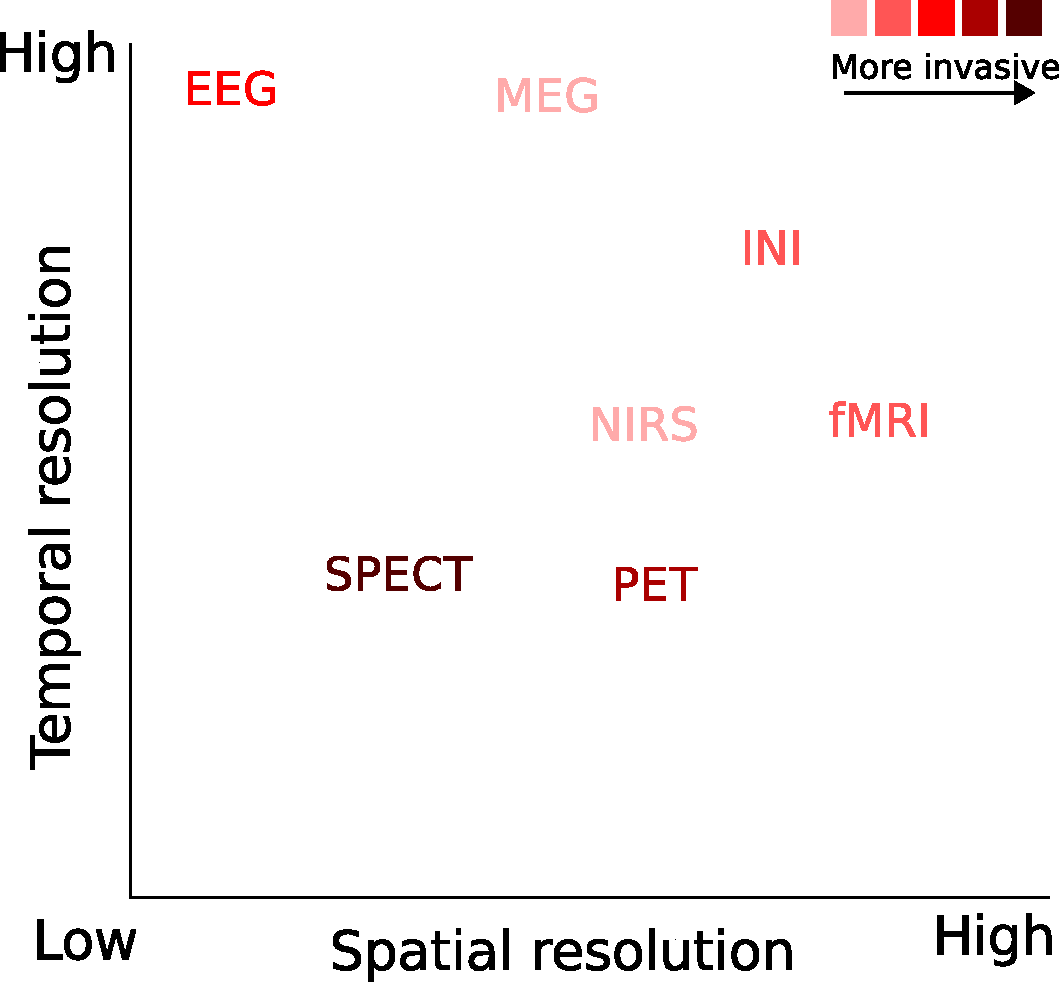
\includegraphics[width=0.6\linewidth]{figures/neuroimaging_methods.pdf}
\end{center}
   \caption[]{Various neuroimaging methods differ in terms of the information they measure. MEG=magnetoencephalography, EEG=electroencephalography, NIRS=near-infrared spectroscopy, PET=positron emission tomography, SPECT=single photon emission tomography, and INI=Inverse imaging, a method to speed up acquisition of fMRI images, ECoG=Electrocorticography, LFP=Local Field Potential.}
   \label{fig:sommaire:neuroimaging_methods}
\end{figure}

Dans cette thèse, nous discuterons des données enregistrées principalement à l'aide de la MEG et de l’EEG. L'EEG et la MEG sont des méthodes d'électrophysiologie permettant d’étudier les propriétés des cellules et tissus biologiques. Les tissus biologiques ont des propriétés électriques dues à la présence d'ions. Tout comme nous pouvons mesurer les tensions dans les appareils électriques, il est également possible de mesurer ces tensions dans les tissus vivants.

L'enregistrement électrophysiologique a l'avantage de mesurer directement l'activité cérébrale, par opposition à une mesure indirecte, ce qui est par exemple le cas de l'IRMf. Les techniques d'imagerie cérébrale se caractérisent par leur résolution temporelle et spatiale, c'est-à-dire l'échelle de temps à laquelle elle peut mesurer l'activité cérébrale, ainsi que la précision de la localisation de la source de l'activité, respectivement. La Figure~\ref{fig:sommaire:neuroimaging_methods} résume les différentes méthodes de neuroimagerie en ce qui concerne leur résolution temporelle et spatiale, mais aussi leur caractère invasif. Ceci est utile pour comprendre pourquoi la MEG/EEG est souvent considéré comme la méthode de choix pour comprendre les fondements de l'activité cérébrale humaine. Bien que l'IRMf soit une autre méthode non invasive, elle mesure le flux sanguin qui est une réponse lente en comparaison à l'activité neuronale ce qui lui confère une résolution temporelle peut élevée.

Il existe un certain nombre de méthodes pour mesurer les potentiels électriques dans le corps humain, la plus connue étant peut-être l'électrocardiographie (ECG) qui est utilisée pour mesurer l'activité électrique du cœur. Les trois méthodes dont nous discutons dans la thèse produisent des séries temporelles multivariées. Un bref résumé de chacune de ces méthodes est présenté ci-dessous.

\paragraph{Électroencéphalographie :} L'EEG est une technique de mesure portable et non invasive inventée dans les années 1920 et utilisée dans plusieurs contextes tels que les BCI, la surveillance médicale et dans l’établissement de diagnostic, ainsi que dans les études cognitives. En électroencéphalographie, un réseau d'électrodes sur un capuchon d’EEG est placé sur le cuir chevelu pour mesurer les tensions par rapport à une électrode de référence. La tension qu'il mesure n'est pas  la résultante d'un seul neurone, mais plutôt le résultat de l'activité électrique de populations de neurones lui conférant une résolution temporelle élevée (de l'ordre des \emph{ms}), quoique la résolution spatiale n'est pas si élevée.

\paragraph{Magnetoencephalography: } Any electric current is associated with magnetic fields as a consequence of Maxwell's theory. 
Therefore, the brain generates tiny magnetic fields which  wrap around the currents according to Maxwell's right hand thumb rule. The field is tiny ($\sim10^{-12}T$) compared to the earth's magnetic field ($\sim10^{-4}T$) and ambient magnetic noise ($\sim10^{-6}T$). Therefore, to measure it, one would need very sensitive electronics and heavy noise cancellation. The measurement itself is done in a magnetically shielded room made of three layers of metals. 
The sensors are superconducting coils which capture the magnetic flux. 
They are immersed in liquid Helium at very low temperatures (around 4 K), so as to lower any loss in signal due to resistance. A typical device contains two types of sensors: gradiometers and magnetometers. While the magnetometer measures the absolute magnitude of magnetic field, the gradiometer measures gradient of the field. \Ac{MEG} has the advantage that the skull does not deteriorate the signal quality as in \ac{EEG}.

\paragraph{Potentiel de champ local (LFP) :}
Le potentiel de champ local est le potentiel électrique qui est enregistré dans l'espace extracellulaire du tissu cérébral. Contrairement à l'EEG, les LFP sont enregistrés en profondeur, à partir du tissu cortical et peuvent donc mesurer des populations de neurones plus localisées. De petites électrodes intracrâniennes sont généralement utilisées pour mesurer ces potentiels, contrairement aux électrodes de grande surface utilisées dans l'EEG.

\section*{Contexte de la thèse}
La thèse se focalise sur les récents mouvements de reproductibilité et de partage des données en neuroimagerie. Elle met l'accent sur la simplification de l'analyse des données grâce à de meilleurs outils pédagogiques et à des méthodes automatisées permettant une analyse reproductible à l'ère des grandes données.

\subsection*{La crise de la reproductibilité}
\label{sec:sommaire:reproducibility_crisis}
Even though thousands of papers are published every year about different aspects of the brain, our understanding of this complex organ has not scaled in proportion. A large part of the reason has been attributed to what is known as the reproducibility crisis~\citep{ioannidis2005most, simmons2011false, button2013power}. %Replication is closely related to the concept of reproducibility which refers to the idea that an experiment produces the same result when performed again under the same conditions. Replication is a stronger condition as it requires similar results or identical conclusion even if there are some minor variations in the experimental procedures. 
Progress in science rests on reproducible experiments. Reproducibility refers to the fact that the findings of an experiment can be regenerated independently if the code, data, and related software was provided. In many fields, however, a large fraction of experiments cannot be reproduced. In psychology, for instance, it was estimated that over half of the papers were not reproducible~\citep{open2015estimating}, and even those which could be reproduced tended to have a weaker effect size compared to the original studies. 

The reasons for unreproducible results can be numerous~\citep{baker20161}, some being: 1) confirmation bias, the tendency to selectively report only experiments that conform to the researcher's pre-existing beliefs, 2) ``p-hacking''~\citep{simmons2011false}, or the tendency to try multiple hypothesis to get a positive result, 3) publication bias or the absence of incentives to publish negative results~\citep{rosenthal1979file}, and 4) pressure to publish. There is now an accepted set of recommendations to address many of these issues: 1) pre-registering research plans to avoid confirmation bias and even report negative results, 2) correct for multiple comparisons, the most conservative method being the Bonferroni correction~\citep{dunn1961multiple}. 

Brain imaging has its own set of issues which can be linked to reproducibility crisis: 

% vul2009puzzlingly
% yendiki2014spurious

\begin{itemize}[noitemsep,partopsep=0pt]
\item \textbf{Power failure:} This is arguably one of the central issues in the reproducibility crisis today and has received by far the most attention. The statistical power of a study refers to the likelihood of discovering an effect of interest, given the sample size. Small sample sizes translate into underpowered studies which means that the chance of a false discovery is high. In order to discover the effect of interest, the study must be appropriately powered.
%
\item \textbf{Comparaisons multiples:} Il s'agit essentiellement d'une manifestation de "piratage" qui résulte du grand nombre de voxels ou de points dans le temps en neuroimagerie. Par exemple, dans la célèbre étude sur le saumon mort~\citep{bennett2009neural}, un effet significatif a été trouvé même si aucun effet n'était attendu simplement parce que les tests d'hypothèse (comparaisons) ont été effectués sur chaque voxel.
%
\item \textbf{Différences dans les versions des logiciels :} Les changements de versions d’un logiciel peut conduire à des résultats différents. Par exemple, dans le cas du logiciel Freesurfer, les différences de volume étaient de l'ordre de $8.8\% \pm 6.6\%$ pour des versions différentes~\citep{gronenschild2012effects}.
%
\item \textbf{Pipelines complexes :} Les pipelines de neuroimagerie impliquent un certain nombre de choix à chaque étape de traitement, et il n'existe actuellement aucun consensus sur la façon de choisir les bonnes étapes d’analyses. Souvent, ces choix méthodologiques ne sont même pas documentés. On estime qu'il y a presque autant de pipelines uniques que d'études~\citep{Carp2012289}.
\item \textbf{Confounds:} There are several methodological confounds such as head movements~\citep{yendiki2014spurious}, anatomy differences, and changes in breathing rate and depth, which can lead to spurious correlations.
\end{itemize}

In Chapter~\ref{chapter:group_study} of the thesis, we will provide concrete guidelines on how to build processing pipelines for \ac{MEG}/\ac{EEG} data. Our contribution will touch upon the issue of complex pipelines, multiple comparison, and differences in software versions in the context of \ac{MEG}/\ac{EEG}. The issue of power failure can be alleviated through data sharing as I will discuss in the next section.

\subsection*{Partage de données}
\label{sec:sommaire:intro_datasharing}
Power failure is essentially a consequence of small datasets. In today's collaborative and data-driven scientific environment, data sharing is useful not only from the perspective of reproducibility but also to build datasets with large sample sizes. With large datasets, it would be possible to tease apart even subtle effects~\citep{smith2017statistical} that were not possible with smaller datasets. Data sharing is beneficial not just from the perspective of replication but also from an economic perspective. Rather than collect new data for every new hypothesis, researchers can now reuse known data for testing the validity of their hypotheses.

Les avantages du partage de données remontent à Newton et à sa théorie de la gravitation~\citep{pointofview2013}. Avant que Newton ait développé sa théorie, un autre astronome anglais, John Flamsteed avait été nommé par le roi pour observer les étoiles et produire des cartes précises pour la navigation dans les mers. Sur une période de 40 ans, Flamsteed a créé un catalogue détaillé qui a triplé le nombre d'entrées dans l'atlas du ciel utilisé précédemment. Lorsque la grande comète de 1680 est apparue deux fois de suite dans le ciel, Flamsteed a utilisé ses données pour suggérer que ce n'était pas deux comètes mais bien la même comète qui s'est d'abord dirigée vers le soleil et s'en est ensuite détournée. Newton s'est d'abord opposé à cette théorie, mais il a changé d'avis plus tard en accédant au catalogue inédit de Flamsteed. La comète s'était en effet avérée être une référence importante pour la théorie de la gravitation de Newton.

Il est difficile d'imaginer à notre époque qu'une théorie aussi fondamentale que les lois de la gravitation aurait pu être guidée par les données. Le partage de données est fondamental non seulement pour la reproductibilité scientifique, mais il constitue également la base de l'apprentissage de modèles plus solides et de l'analyse comparative de nouveaux algorithmes. Par conséquent, dans le domaine de l'apprentissage automatique, les percées récentes ont été alimentées par l'augmentation du partage de données et du calcul. Cela inclut la croissance récente de l'apprentissage profond~\citep{deng2009imagenet}, l'apprentissage Q~\citep{watkins1992q, bellemare2013arcade}, le traitement du langage naturel pour la traduction du langage~\citep{halevy2009unreasonable}, la reconnaissance vocale~\citep{paul1992design}, et même le modèle du mélange d'experts~\citep{jacobs1991adaptive} pour IBM Watson~\citep{ferrucci2010building}. La maxime ``plus de données battent un algorithme plus intelligent''~\citep{domingos2012few} a remarquablement bien résisté à travers les disciplines et les âges.

Bien sûr, les neuroscientifiques commencent à prendre conscience de l'importance du partage de données. Récemment, les données neuronales ont commencé à être partagées par le biais de consortiums internationaux~\citep{van2013wu, ollier2005uk}, de dépôts de données~\citep{poldrack2013toward, gorgolewski2015neurovault} et d'articles sur les ensembles de données dans des revues ciblées. Pourtant, il y a encore un gros écart entre  l'idéal du partage de données et ce qui est pratiqué. Les expériences de neuroimagerie sont souvent très compliquées et il ne suffit pas de partager simplement les données, mais aussi les métadonnées et les informations concernant les protocoles expérimentaux dans un format bien structuré. En l'absence de cette information, les données partagées ne sont pas réutilisables de la même manière que les programmes peu commenté, mal structurés, et compliqués ne sont pas utiles même s'ils sont partagés publiquement. Il n'y a pas de consensus accepté au sein de la communauté sur les pratiques de partage des données et il est nécessaire d'établir une norme.
Au Chapter~\ref{chapter:group_study}, nous présenterons une nouvelle norme connue sous le nom de BIDS, qui vise à combler cet écart. Il s'agit d'un effort de collaboration entre les développeurs de logiciels et les neuroscientifiques de divers laboratoires afin d'établir un consensus sur les normes et d'élaborer des outils pour faciliter l'adoption de la norme.

\subsection*{Automatisation}
\label{sec:sommaire:automation}

En 2014, Nature a publié un article audacieux~\citep{hayden2014automated} qui décrivait une vision de l'avenir de la science : des laboratoires automatisés qui enregistrerait de façon autonome chaque détail d'une expérience, ce qui mènerait à une recherche moins coûteuse, plus efficace et plus fiable. Bien qu'il décrive de nombreux laboratoires de biologie qui automatisent des expériences, les avantages de l'automatisation dans le domaine de la neuroimagerie ne sont pas encore largement reconnus. L'automatisation permet non seulement de gagner du temps, mais aussi de rendre la recherche plus reproductible, comme cela a été noté dans un guide récent pour améliorer la transparence et la reproductibilité de la recherche en neuroimagerie~\citep{gorgolewski2016practical}. Les auteurs soulignent que le travail manuel peut sembler facile à première vue, si l'analyse ne doit être effectuée qu'une seule fois. Toutefois, ce n'est pas toujours le cas, car ``assez souvent, au cours d'un projet, les paramètres sont modifiés, les sujets sont changés et les étapes de traitement doivent être ré-exécutées. C'est une situation dans laquelle le fait d'avoir un ensemble de scripts capables d'exécuter automatiquement toutes les étapes de traitement au lieu de s'appuyer sur des interventions manuelles peut être vraiment payant.'' Comme les grands ensembles de données deviennent de plus en plus courants en neuroimagerie, l'automatisation deviendra en effet une nécessité plutôt qu'un luxe.

En neuroimagerie, il existe en fait plusieurs voies d'automatisation :
\begin{itemize}[noitemsep,nolistsep,nosep]
\item \textbf{Réduire l'interactivité :} Si les interfaces graphiques interactives sont d'excellents outils pour la navigation dans les données, elles sont insuffisantes lorsqu'il s'agit d'étendre l'analyse à des dizaines et des centaines de sujets, ce qui est nécessaire pour une étude suffisamment puissante.

\item \textbf{Réglage des paramètres :} La plupart des algorithmes, bien que scénarisés, nécessitent encore des hyperparamètres à être réglés. Ces hyperparamètres peuvent être le nombre de composants ICA à choisir ou les paramètres de régularisation, et peuvent varier d'un sujet à un autre.
%This could be the number of trials to perform in an experiment, the number of components to select in a \ac{PCA} decomposition, or the regularization parameter in inverse solvers.
\item \textbf{Annotation et étiquetage :} Une grande partie des données de neuroimagerie disponibles n'est pas étiquetée ou, au mieux, est faiblement étiquetée. C'est parce que les annotations d'experts sont coûteuses et ne peuvent pas être financées par la foule. Les outils automatisés basés sur l'apprentissage non supervisé peuvent jouer un rôle majeur en ce sujet.
%
\item \textbf{Contrôle de qualité :} Actuellement, le contrôle de qualité est effectué manuellement en inspectant les données pour repérer les valeurs aberrantes. Même si l'inspection des données ne peut pas être négligée, elle peut être effectuée plus efficacement grâce à la documentation automatisée des analyses de données et des rapports tels que le carnet de notes Jupyter et le rapport Web MNE~\citep{dengemann2015conc}. En parallèle, des analyses de tendances statistiques avancées comme dans le projet ``Automated Statistician''~\citep{duvenaud2013structure} peuvent être utilisées pour créer des résumés.
\end{itemize}

There have been some steps taken in this direction, most notably the Neurosynth platform~\citep{yarkoni2011large} which facilitates large-scale meta analysis. Meta analysis typically combine results from multiple studies, and in this case, it is the brain activation maps from different studies which are combined by using machine learning methods. On the software side, the Freesurfer software package~\citep{dale-fischl-etal:99, fischl-serena-etal:99} provides a \code{recon-all} command that performs cortical segmentation automatically without any human intervention. In MNE, this philosophy is now being adopted starting with automated covariance estimation~\citep{engemann2015automated_new}.

In this thesis, we will consider an algorithm that automatically annotates artifacts in the data~\citep{jas2016automated, jas2017autoreject}. This is a first step that any \ac{MEG}/\ac{EEG} processing pipeline has to go through but it is often done manually. A reason for this is that existing algorithms are not designed to be \emph{transparent}. Since for most scientists, the key to new insights is an artifact-free dataset, they would rather spend extra effort in doing this manually rather than depend on a generic algorithm which is difficult to interpret. %However, this is problematic as it can lead to a selection bias: they might end up rejecting data segments which helps them confirm their hypothesis. 
Merely based on anecdotal reports, this process can take up to a week even for a moderately sized study of 10--20 subjects.

This is what led us to propose \emph{autoreject}, which we describe in Chapter~\ref{chapter:autoreject}. It is an algorithm which can be used to mark bad segments of the data. The key insight is that, often certain sensors in the device are intermittently corrupted rather than continuously. We validate our algorithm against 3 benchmarks on the \ac{HCP} dataset~\citep{larson2013adding} which is manually annotated with bad segments. In the process, our work also represents one of the first attempts at reanalyzing the MEG component of the HCP dataset.

\subsection*{Representation learning for data-driven discovery}
\label{sec:sommaire:representation_learning}
Depuis l'invention de l'EEG dans les années 1920, les scientifiques ont découvert plusieurs modèles différents d'oscillation cérébrale tels que les ondes alpha, les complexes K et les rythmes mu. Les oscillations et les interactions entre eux ont servi de biomarqueurs pour différentes fonctions et pathologies du cerveau. Les ondes alpha ont été impliquées dans l'attention, les complexes K dans le sommeil et le rythme mu dans l'activité motrice.

Considering the complexity of the human brain, clearly these waveforms represent only a fraction of the cognitive functions that the brain may perform. As a result of the wealth of data now available through the data sharing movement described in Section~\ref{sec:intro_datasharing}, the future neuroscientist will be able to mine such waveforms from large datasets. Imagine if neuroscientists had at their disposal a tool similar to Google Photos\footnote{\url{https://photos.google.com/}}. In the same way that Google Photos can automatically find faces and group photos, such tools will be able to find prototypical oscillations and cluster the data using them. Clicking on any of these waveforms would retrieve the data associated with them.

\begin{figure}[t]
\begin{center}
   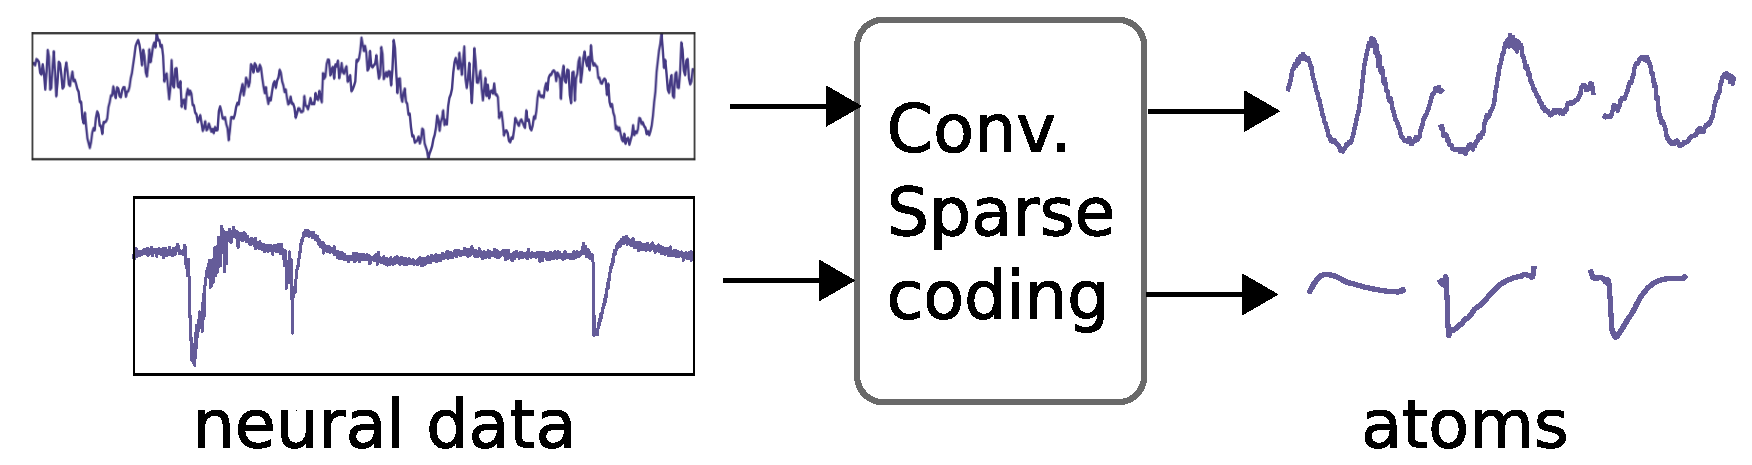
\includegraphics[width=0.85\linewidth]{figures/schema.pdf}
\end{center}
   \caption[]{Une illustration de la façon dont le codage à faible densité convolutionnelle peut être utilisé pour extraire automatiquement les formes d'onde prototypiques.}
   \label{fig:sommaire:csc_schematic}
\end{figure}

However, photos are inherently different from neural data. First, neural data can be buried in noise and corrupted by high amplitude artifacts. Second, images are labelled owing to crowdsourced data as in the case of  Imagenet~\citep{deng2009imagenet}, but neural data is not. 
Expert annotations in the case of neural data are not easily available.
Finally, it is spatiotemporal data with different dynamics from the 3D world that photos capture. This is where \ac{CSC} can play a role by extracting prototypical features from the data, as shown in Figure~\ref{fig:sommaire:csc_schematic}. It is an unsupervised algorithm from computer vision, which can learn shift-invariant dictionaries of prototypical waveforms (atoms) from the data using the convolution operations. For a more comprehensive background on \ac{CSC}, the reader may read Section~\ref{sec:background_dict_learning} later in this chapter.

\ac{CSC} algorithms do not approximate the signal using Fourier (or sinusoidal) basis. While this is the conventional technique for extracting signals buried in noise, the approximation can degrade the shape of the signal, which can be a biomarker in many clinical diseases~\citep{cole2017brain}. As an example, even with a large number of sinusoids from the Fourier basis, the edges of a square wave cannot be approximated well. Indeed, the imperfect approximation around such edges is what is often termed as ringing artifacts in signal processing contexts. Of course, transients can be better approximated using wavelets but it is clearly not sufficient for other shapes of data. Rather than fix the basis to be Fourier or wavelet, the \ac{CSC} approach is to learn \emph{both} the basis and the coefficients.

In our work presented in Chapter~\ref{chapter:alphacsc}, we extend conventional \ac{CSC} algorithms for heavy-tailed noise. We reformulate the optimization problem as a \ac{MAP} inference with an alpha-stable distribution to replace the reconstruction loss. Our results show that this kind of algorithm is robust to the presence of artifacts and can be used to uncover temporal structures from neural signals, even those involving nested oscillations.

\section*{Chapter~\ref{chapter:bids}: Brain Imaging Data Structure (BIDS)}

\begin{figure}[htb!]
\begin{center}
   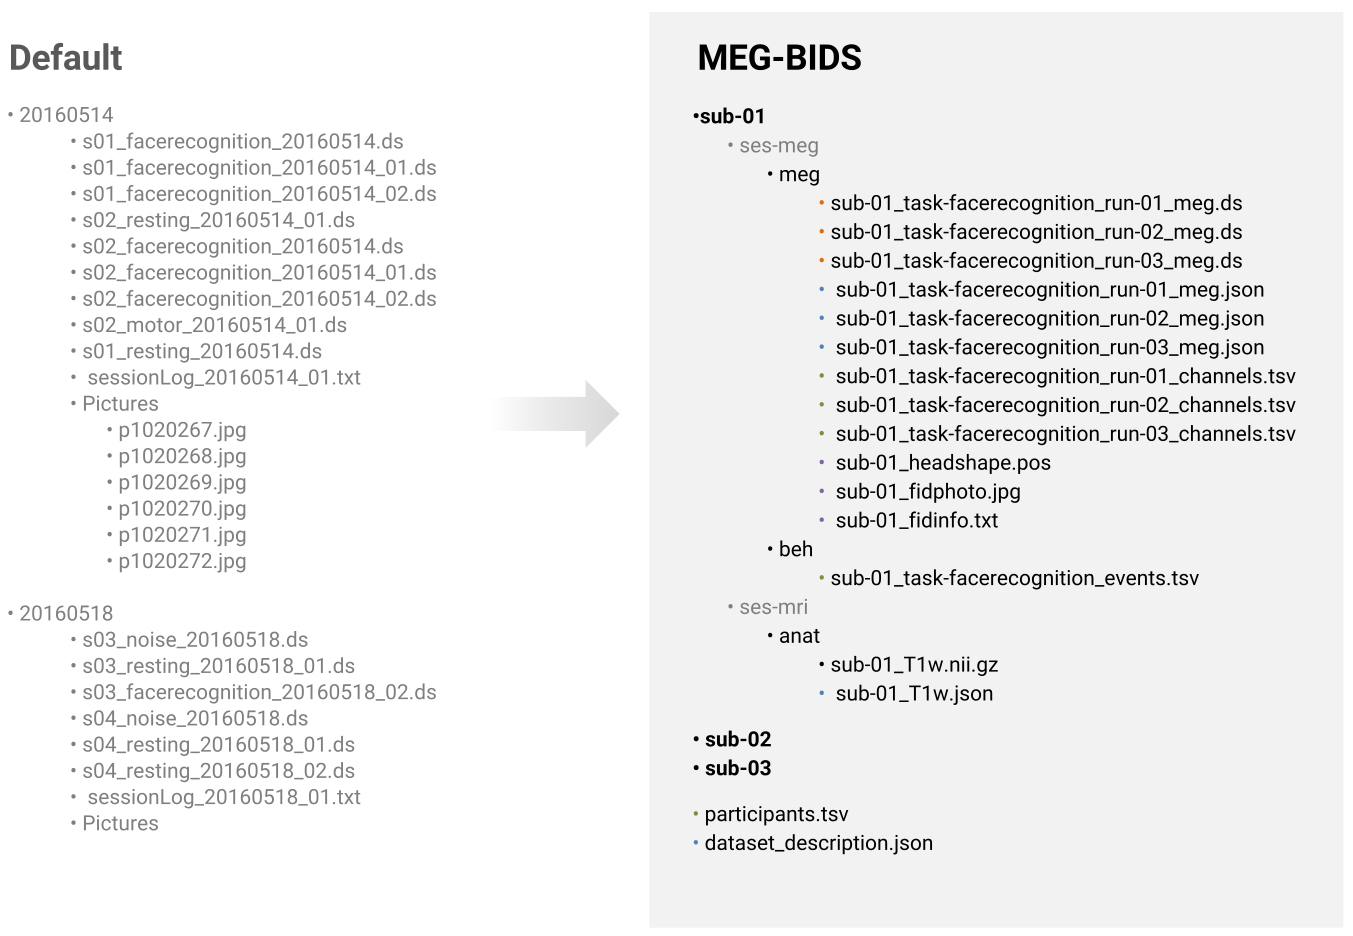
\includegraphics[width=\linewidth]{figures/bids_organization.png}
\end{center}
   \caption[]{Schéma d'organisation des données BIDS-MEG : Gauche : un schéma typique d'organisation des données par défaut où les dossiers sont organisés par date de session et contiennent différentes exécutions pour un participant donné dans une étude. Droite: BIDS-MEG organise les données par étude, puis par participant (sujet), suivi de la modalité, puis des sessions et finalement des runs. Notez les fichiers latéraux qui sont présents à tous les niveaux de la hiérarchie des données et documentez facilement le contenu des métadonnées.}
   \label{fig:sommaire:BIDS-MEG-organization}
\end{figure}
Du point de vue de la reproductibilité, le partage des données est d'une importance capitale. Le code de partage en soi ne permet pas la reproductibilité si les données qui l'accompagnent ne sont pas disponibles et sont coûteuses à acquérir. La réanalyse d'un ensemble de données est cependant utile non seulement du point de vue de la reproductibilité, mais aussi pour découvrir de nouveaux effets qui étaient auparavant négligés. En même temps, plus les données sont partagées, plus la taille de nos échantillons sera grande, ce qui nous permettra de mener des études avec une plus grande puissance statistique. En effet, la faible puissance statistique est l'une des principales raisons de la crise de la reproductibilité.

While data sharing in neuroscience is on the rise, the amount of data reuse is still limited. For example, since the release of the Human Connectome Project (HCP)~\citep{larson2013adding} MEG data in 2013, there have been very few instances of reusing this data. At the time of writing this thesis, we had only one or two documented cases~\citep{jas2017autoreject} of reusing the HCP data. Even in these cases, the effort has mostly been limited to reproducing results rather than testing new hypotheses. This clearly represents a gap between the ideal and the practice of data sharing. 

% Clearly, sharing data is not a panacea as the tools, skills and resources to process such large datasets is currently missing in typical laboratories. Perhaps the most important roadblock is standardization of metadata.

Neuroimaging experiments are often complicated involving different  cognitive tasks (auditory, visual, somatosensory \emph{etc.}), different acquisition parameters (sampling frequency, number of sensors and their location, measurement device \emph{etc.}), and population parameters (subject's gender, age \emph{etc.}). All of this metadata is necessary information to successfully reanalyze the data. Unfortunately, historically there has been a lack of consensus amongst different labs and industrial manufacturers as to what constitutes useful metadata. This points to the need for establishing standards. While on a first glance, this may appear to be unnecessary bureaucratic red tape, in fact standards exist in almost all facets of our life. 

Apart from the meta information that is stored with the data, the data itself is stored amongst one of 10--20 different file formats and at different stages of processing. While there have been some efforts previously to standardize data structures~\citep{gibson2009minimum, grewe2011bottom, stoewer2013singlefile, teeters2015neurodata, bigdely2016preparing}, it has not gained wide acceptability. Designing a new standard is tricky as it requires gaining a community consensus. At the same time it must strike the right balance between rigidity for efficiency and flexibility for adapting to future technologies. 

The \ac{BIDS} format~\citep{gorgolewski2016brain} is indeed designed with these considerations in mind. 
The standard involves a hierarchy of folders to describe the imaging technology used, the name of the subject, and the date of the experiment. 
At each level of hierarchy, files are accompanied by sidecar \code{json} files describing the metadata. 
A \code{json} file is an easy to parse text file that contains key and value pairs, so that it has the advantage of being machine and human readable at the same time. 
These files follow an \emph{inheritance principle}, that is, a field described in a \code{json} file in a higher level of the hierarchy will be automatically propagated downstream. 
The main BIDS specification is accompanied by extension specifications which describe specific aspects to describe different modalities.
%
En même temps, la norme n'existe pas isolément. Le consortium BIDS fournit également un écosystème croissant d'outils pour convertir les ensembles de données dans un format compatible BIDS et pour valider les données afin qu'elles soient conformes à la norme.
%
In this work, we presented a significant extension of \ac{BIDS} to support the specific aspects of \ac{MEG} data. \Ac{MEG}, as we know, provides direct measurement of brain activity with millisecond temporal resolution and unique source imaging capabilities. So far, \ac{BIDS} has provided a solution to structure the organization of \ac{MRI} data. Despite the lack of standard data format for \ac{MEG}, BIDS-MEG is a principled solution to store, organize and share the typically-large data volumes produced. It builds on \ac{BIDS} for \ac{MRI}, and therefore readily yields a multimodal data organization by construction. This is particularly valuable for the anatomical and functional registration of \ac{MEG} source imaging with \ac{MRI}. With BIDS-MEG and a growing range of software adopting the standard, the \ac{MEG} community has a solution to minimize curation overheads, reduce data handling errors and optimize usage of computational resources for data analysis. The standard also includes well-defined metadata to facilitate future data harmonization and sharing efforts, and extensions to other electrophysiological data modalities.

\subsection*{Outils logiciels}
Dans le cadre de cet effort, j'ai participé aux discussions pour décider de la norme. En même temps, j'ai développé l'extension MEG du validateur BIDS. Développé en javascript à l'aide de “nodejs”, il peut être packagé pour fonctionner dans le navigateur (Google Chrome). Une version en ligne de commande est également fournie afin qu'elle puisse être utilisée dans l'analyse par script. Le validateur effectue plusieurs contrôles de santé mentale sur les ensembles de données pour s'assurer qu'ils sont compatibles avec BIDS. Cela comprend l'utilisation d'expressions régulières pour vérifier les noms de fichiers et de schémas de notation d'objets JavaScript (JSON) pour s'assurer que les fichiers de métadonnées sont normalisés par type de données.

Afin de faciliter l'adoption du format BIDS, j'ai également contribué au code Python qui est utilisé pour convertir les jeux de données existants en jeux de données compatibles BIDS. Le code peut être trouvé ici : \url{https://github.com/mne-tools/mne-bids}. 

Pour une description plus détaillée de la spécification BIDS-MEG, des exemples de données, des ressources et des commentaires, veuillez visiter le site \url{http://bids.neuroimaging.io}.

\section*{Chapter~\ref{chapter:group_study}: A reproducible M/EEG group study}

In the previous section, we discussed how data sharing can be facilitated using the \ac{BIDS} for \ac{MEG}. This is taking us one step closer to the goal of reproducibility. However, reproducibility is not achieved by merely sharing more data with the hope that this will solve all problems. As noted in \citet{baker20161}, one of the best solutions to foster reproducible science is not a technical one, but an educational one. This is of course true for statistics, where there is an urgent need to clarify and educate researchers about the statistical tools required in neuroscience. But it is now increasingly important also for academic software.

In recent years, free academic toolboxes have gained increasing prominence in \ac{MEG} analysis as a means to disseminate cutting edge methods, share best practices between different research groups and pool resources for developing essential tools for the \ac{MEG} community. Teaching events are regularly held around the world where the basics of each toolbox are explained by its  developers and experienced power users. There are however, knowledge gaps that need to be addressed. First, most teaching examples only show analysis of a single ‘typical best’ subject whereas most real MEG studies involve analysis of group data. It is then left to the researchers in the field to figure out for themselves how to make the transition and obtain significant group results. Secondly, we are not familiar with any examples of fully analyzing the same group dataset with different academic toolboxes to assess the degree of agreement in scientific conclusions and compare strengths and weaknesses of various analysis methods and their independent implementations.

\section*{Methods}
To address this very issue, a workshop was organised by the lead developers of six most popular free academic MEG toolboxes at Biomag 2017. This work is a follow up to the workshop, which presents the contribution of the MNE software team, and will be published in \emph{Frontiers in Neuroscience, section Brain Imaging Methods}. This study presents the results obtained by the reanalysis of an open dataset from \citet{wakeman2015multi} using the MNE software package. The analysis covers preprocessing steps, quality assurance, sensor-space analysis of evoked responses, source localization, and statistics in both sensor and source space. Results with possible alternative strategies are presented and discussed at different stages such as the use of high-pass filtering versus baseline correction, tSSS versus \ac{SSS}, the use of a minimum norm inverse versus \ac{LCMV} beamformer, and the use of univariate or multivariate statistics. 


\section*{Results}

This aims to provide a comparative study of different stages of \ac{MEG}/\ac{EEG} analysis pipeline on the same dataset, with open access (\url{https://github.com/mne-tools/mne-biomag-group-demo}) to all of the scripts necessary to reproduce this analysis. An example of such a reanalysis figure is shown in Figure~\ref{fig:sommaire:grand_average} which shows the evoked response for one EEG sensor. Indeed, we are not only able to reproduce the results from \citet{wakeman2015multi} but also tease apart the factors that could lead to different results. The work ends with a set of recommendations based on the lessons we learned from this reanalysis exercise.

\begin{figure}[htb]
  \centering
  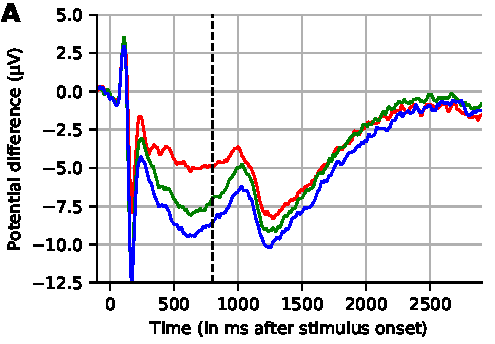
\includegraphics[width=0.7\linewidth]{figures/grand_average_highpass-NoneHz.pdf}\\
  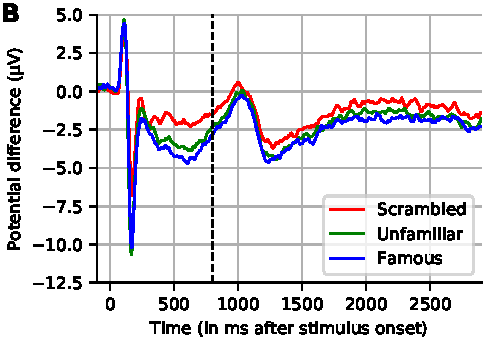
\includegraphics[width=0.7\linewidth]{figures/grand_average_highpass-1Hz.pdf}
\caption[]{Grand averaged evoked response across 16 subjects for channel EEG065.
(A) No highpass filter. (B) Highpass filtered at 1.0 Hz. Note that, similar to (A), the results reported by \cite{wakeman2015multi} (dashed line at 800 ms indicates where their plot stopped) show large drifts, but these return to near-baseline levels toward the end of a sufficiently long interval (here, 2.9 seconds) even without applying a highpass filter.}
\label{fig:sommaire:grand_average}
\end{figure}  

\clearpage

\section*{Chapter~\ref{chapter:autoreject}: Automated artifact rejection for M/EEG}

In the previous section, we discussed the reproducibility challenges when performing group studies in \ac{MEG} and \ac{EEG}. One way to improve reproducibility is automation. and we briefly touched upon an algorithm for automating detection of bad data segments, known as \emph{autoreject}.

%copy pasted abstract below
In this section, we will present this algorithm which rejects and repairs bad trials in \ac{MEG} and \ac{EEG} signals. Annotating bad segments in the data is perhaps one of the most time consuming aspects of data processing in electrophysiology. Currently, it is either done manually, or using automated black-box algorithms (\textit{e.g.,} RANSAC~\citep{bigdely2015prep}, FASTER~\citep{nolan2010faster}, SNS~\citep{de2008sensor}). The manual approach is often subjective with often no clear consensus on what constitutes a corrupted data segment. Therefore, reanalysis is not only manually demanding but can also lead to problems in reproducibility. On the other hand, the automated methods are controlled by parameters that are not straightforward to tune. In the case of failure, it is not always obvious what caused the method to fail and how it can be corrected. As a result, one is left with no choice but to exclude the data from further analysis.

\subsection*{Methods}

\begin{figure}[htb]
	\centering
	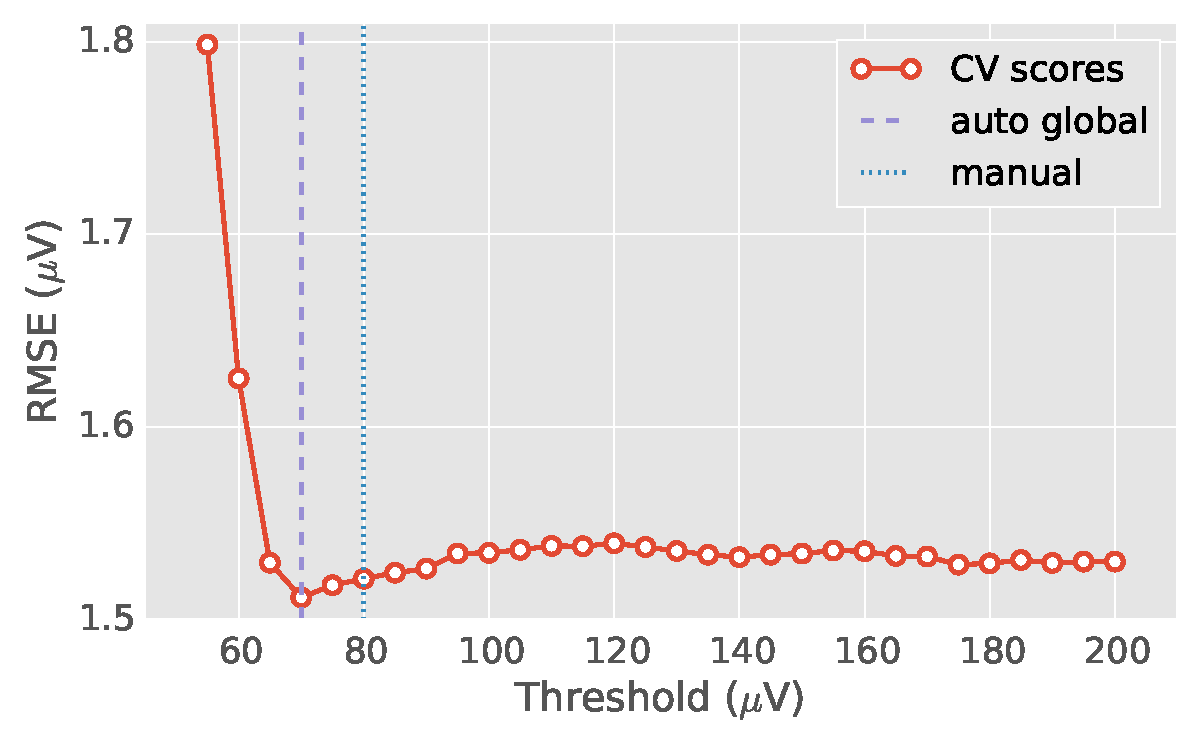
\includegraphics[width=0.8\linewidth]{figures/figure1.pdf}
    \caption[]{Cross-validation error as a function of peak-to-peak rejection threshold on one EEG dataset. The root mean squared error (RMSE) between the mean of the training set (after removing the trials marked as bad) and the median of the validation set was used as the cross-validation metric (Section~\ref{sec:auto_global}). The two insets show the average of the trials as ``butterfly plots" (each curve representing one sensor) for very low and high thresholds. For low thresholds, the RMSE is high because most of the trials are rejected (underfit). At high thresholds, the model does not drop any trials (overfit). The optimal data-driven threshold (\emph{autoreject, global}) with minimum RMSE is somewhere in between. It closely matches the human threshold.}
    \label{fig:sommaire:cross_val}
\end{figure}

This led us to develop a method based on design choices motivated by ease of interpretation and diagnosis. 
The method we propose capitalizes on cross-validation (Figure~\ref{fig:sommaire:cross_val}) in conjunction with a robust evaluation metric to estimate the optimal peak-to-peak threshold--a quantity commonly used for identifying bad trials in \ac{MEG}/\ac{EEG}. 
The key insight is that the training and validation sets are more similar when the data does not contain outliers than when it does. Thus a threshold that minimizes the cross-validation error is one which removes the outliers. 
Indeed, as we see in Figure~\ref{fig:sommaire:cross_val}, for very low thresholds, too many trials are removed which results in a noisy average, whereas for very high thresholds, the outliers are not removed. 
The optimum is somewhere in between which can be estimated by minimizing the cross-validation error.

This approach is then extended to a more sophisticated algorithm which estimates this threshold for each sensor yielding trial-wise bad sensors. Depending on the number of bad sensors, the trial is then repaired by interpolation or by excluding it from subsequent analysis. For efficiency reasons, we use Bayesian optimization which is a well-known technique for hyperparameter optimization. All steps of the algorithm are fully automated thus lending itself to the name \emph{autoreject}. Crucially, the algorithm is even able to deal with sensors that are locally corrupted, which is quite often the case for \ac{EEG} data.

\subsection*{Results}

\begin{figure}[htb]
    \centering
    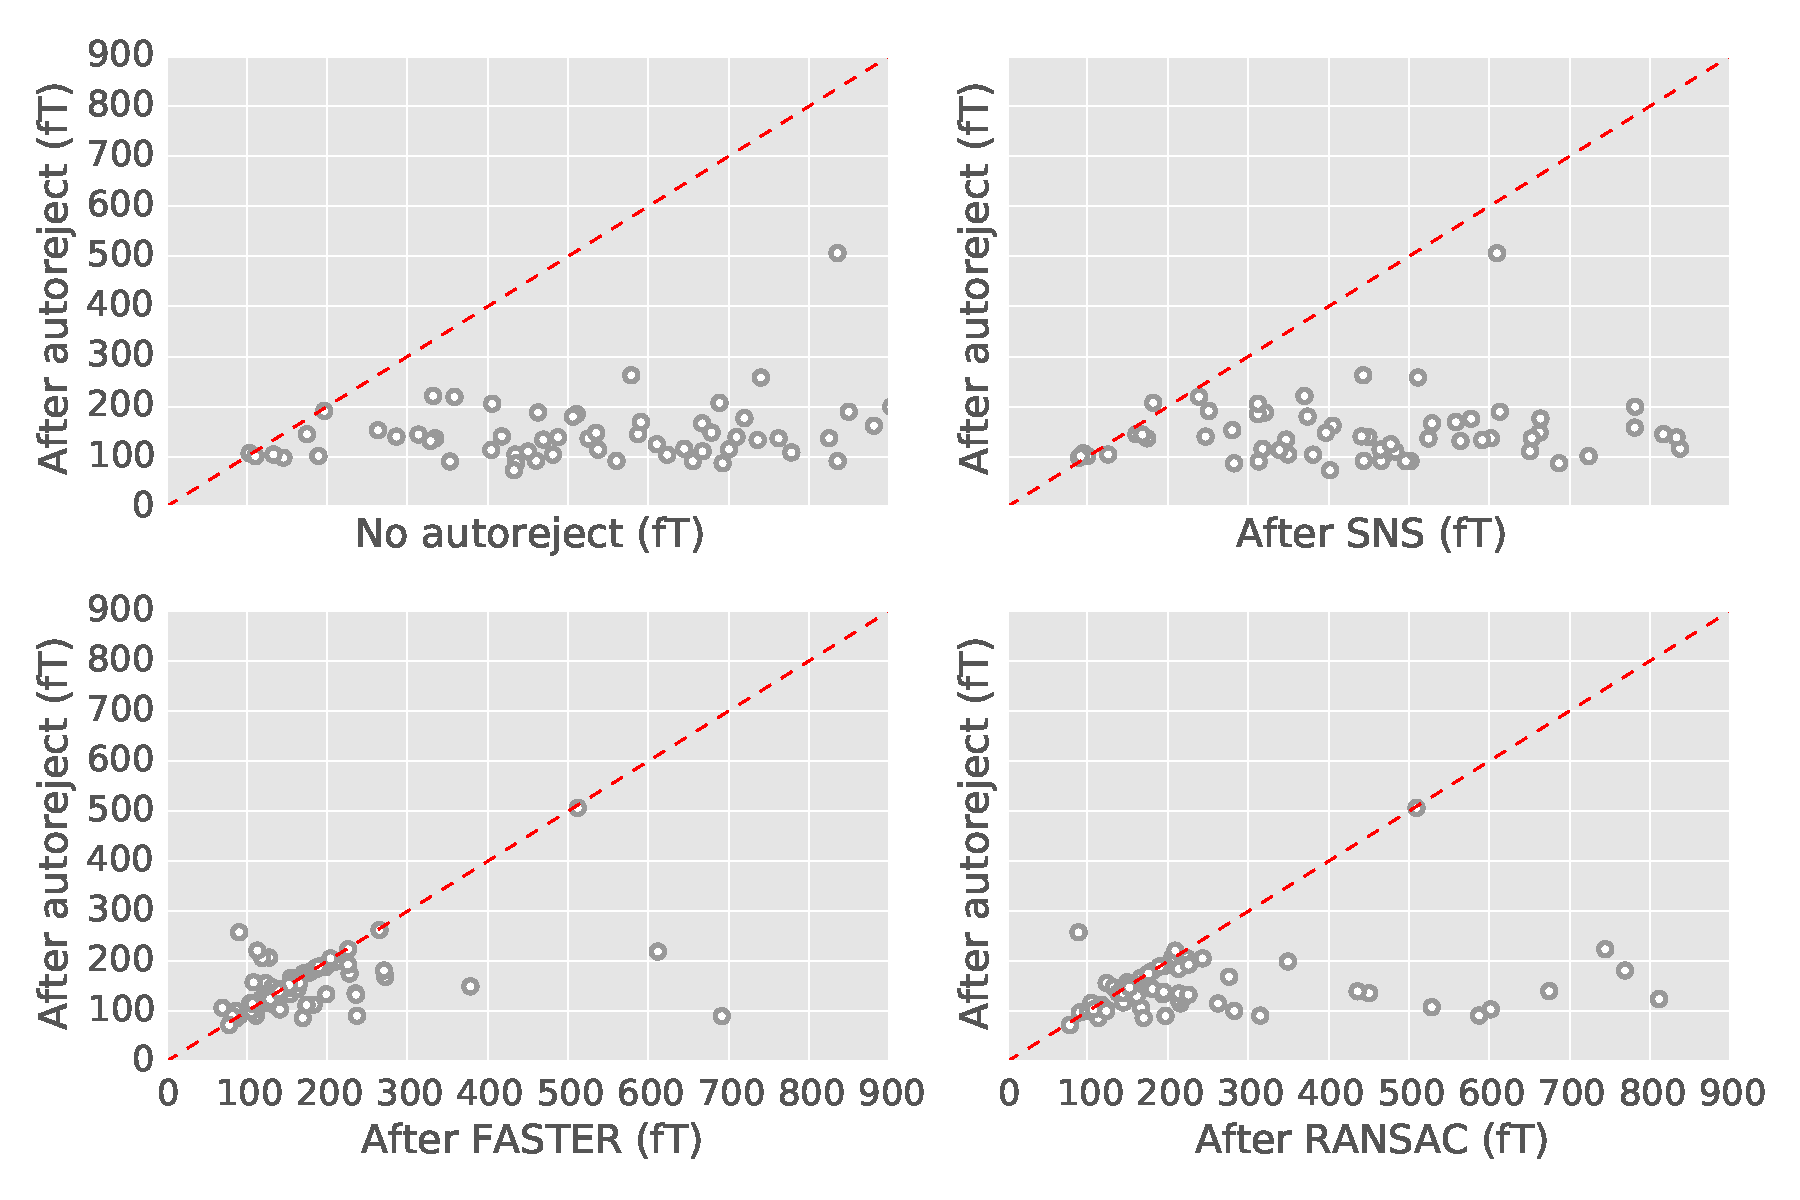
\includegraphics[width=\linewidth]{figures/figure4.pdf}
    \caption[]{Scatter plots for the results with the HCP data. For each method, the $\infnorm{\cdot}$ norm of the difference between the HCP ground truth and the method is taken. Each circle is a subject. (A) \textit{autoreject (local)} against no rejection, (B) \textit{autoreject (local)} against Sensor Noise Suppression (SNS) (SNS), (C) \textit{autoreject} against FASTER, (D) \textit{autoreject (local)} against RANSAC. Data points below the dotted red line indicate subjects for which \textit{autoreject (local)} outperforms the alternative method.}
    \label{fig:sommaire:hcp_scatter}
\end{figure}

\begin{figure}[htb!]
	\centering
	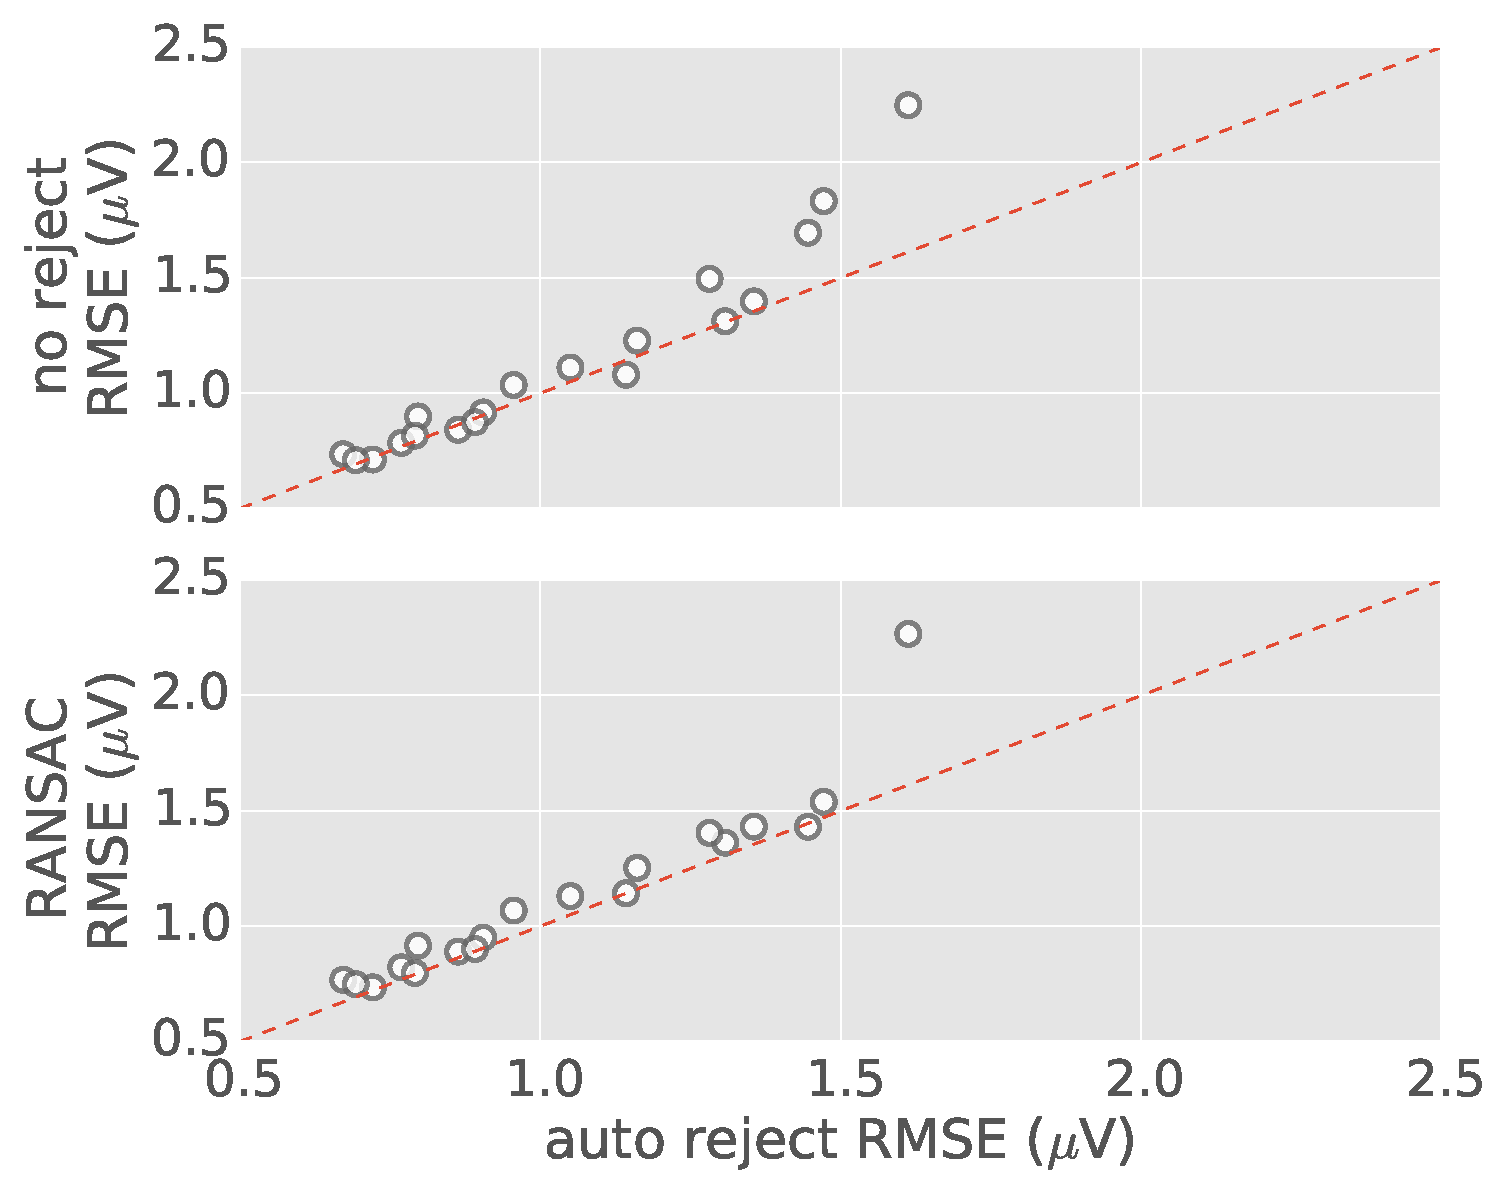
\includegraphics[width=0.9\linewidth]{figures/figure5.pdf}
    \caption[The evoked response (average of data across trials) on three different datasets before and after applying \emph{autoreject}]{The evoked response (average of data across trials) on three different datasets before and after applying \emph{autoreject} --- the MNE sample data, the HCP data and the EEG faces data. Each sensor is a line on the plots. On the left, manually annotated bad sensors are shown in red. The algorithm finds the bad sensors automatically and repairs them for the relevant trials. Note that it can even fix multiple sensors at a time and works for different modalities of data acquisition.}
    \label{fig:sommaire:sample_evoked}
\end{figure}

In order to assess the practical significance of the algorithm, we conducted extensive validation and comparisons with state-of-the-art methods on four public datasets containing \ac{MEG} and \ac{EEG} recordings from more than 200 subjects. The comparisons include purely qualitative efforts (Figure~\ref{fig:sommaire:sample_evoked}) as well as quantitatively benchmarking against human supervised (Figure~\ref{fig:sommaire:hcp_scatter}) and semi-automated preprocessing pipelines. Our qualitative comparisons showed that \emph{autoreject} was able to annotate and repair bad segments satisfactorily for different datasets. Indeed, the algorithm allowed us to automate the preprocessing of \ac{MEG} data from the \ac{HCP} going up to the computation of the evoked responses. The automated nature of our method minimizes the burden of human inspection, hence supporting scalability and reliability demanded by data analysis in modern neuroscience.

\section*{Chapter~\ref{chapter:alphacsc}: Temporal representation learning}

So far, we studied automation in neuroimaging with the objective of enabling scalable data analysis and reproducibility. While  reproducibility and large-scale data analysis allow us to consolidate upon existing studies, \emph{per se} they are not tools to uncover new and interesting phenomena. In this section, we will explore this dimension of automation using what is known as \emph{representation learning}.

Representations are the building blocks of signal processing. It is quite easy to convince ourselves of this fact, if we simply use a Fast Fourier Transform (FFT) to filter data. When we are using an FFT, we are in effect, decomposing the signal into a sum of sinusoids of varying frequencies. If we are interested in a time-frequency analysis, a common choice of representation for neurosience signals consists in using Morlet wavelets.

Traditionally, the choice of representation has been mainly driven by analytical concern and ease of mathematical manipulation. However, the recent surge of deep learning has ignited an interest in data-driven representations. It is because good representations  that compactly capture the properties of the data are essential for efficient and accurate learning systems. In computer vision, for instance, handcrafted features such as SIFT~\citep{lowe1999object} and GIST descriptors~\citep{oliva2001modeling}, Deformable Parts Model (DPM)~\citep{felzenszwalb2010object}, Histogram of Oriented Gradient (HOG)~\citep{dalal2005histograms} \emph{etc.} had been the norm, before it was realized that unsupervised learning and autoencoders performed much better.

Today, unsupervised learning is used as a first step for a supervised learning task in computer vision. Representation learning, by itself, is perhaps not as interesting, except for diagnostic visualizations in deep learning~\citep{zeiler2014visualizing}. Despite this, there has always been an interest in understanding representations in the human brain (visual system particularly), as it was thought that this would help us build better learning systems. One of the pioneers in this area of research is Bruno Olshausen, whose work on dictionary learning~\citep{olshausen1996emergence} demonstrated that Gabor patches are indeed fundamental to natural images, similar to the ones that Hubel and Wiesel~\citep{hubel1962receptive, marcelja1980mathematical} found in the cat visual cortex, and to what is used in GIST features. Barring this line of studies, the learned representation itself is not considered as meaningful as performance metrics like the prediction score or reconstruction loss. However, in the case of neural signals, we realized that this is not the case and the fidelity of the representation is in itself interesting. Indeed, the shape of the signal is a crucial biomarker in many clinical applications for neuroscience~\citep{cole2017brain}. 

A parallel development in the field of neuroimaging has been the rise in interest for learning prototypical shapes which are shift invariant~\citep{jost2006motif, barthelemy2013multivariate, brockmeier2016learning, hitziger2017adaptive}. It is motivated by the fact that existing approximations using the Fourier basis often distorts the signal. There is, for example, a debate regarding the type of filters that should be used (See Section~\ref{sec:group_study_temporal_filtering} and \cite{widmann2015digital,parks1987digital,ifeachor2002digital, gotz-etal:15}). 
Even though some success has been reported
with these algorithms in neuroimaging, they are limited in applicability due to their heuristic nature.
Remarkably, there has been so far very little cross-pollination of ideas between the computer vision and neuroimaging communities on these sparse coding aspects. 
Our work is an attempt to bridge this gap. 
We propose a model which builds upon existing shift-invariant sparse coding models to be able to handle heavy-tailed noise and artifacts. It assumes positivity of the coefficients to account for the fact that an atom does not change polarity over time. 

\subsection*{Methods}

\begin{figure}[htb]
    \centering
     \subfigure[$K=10$, $L=32$.]{
     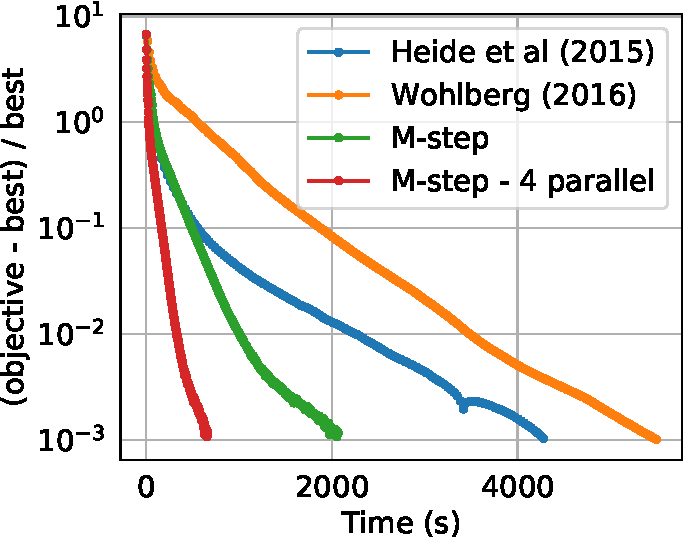
\includegraphics[width=0.5\linewidth]{figures/relative_10_32.pdf}} \\
     \subfigure[Time to reach a relative precision of 0.01.]{
     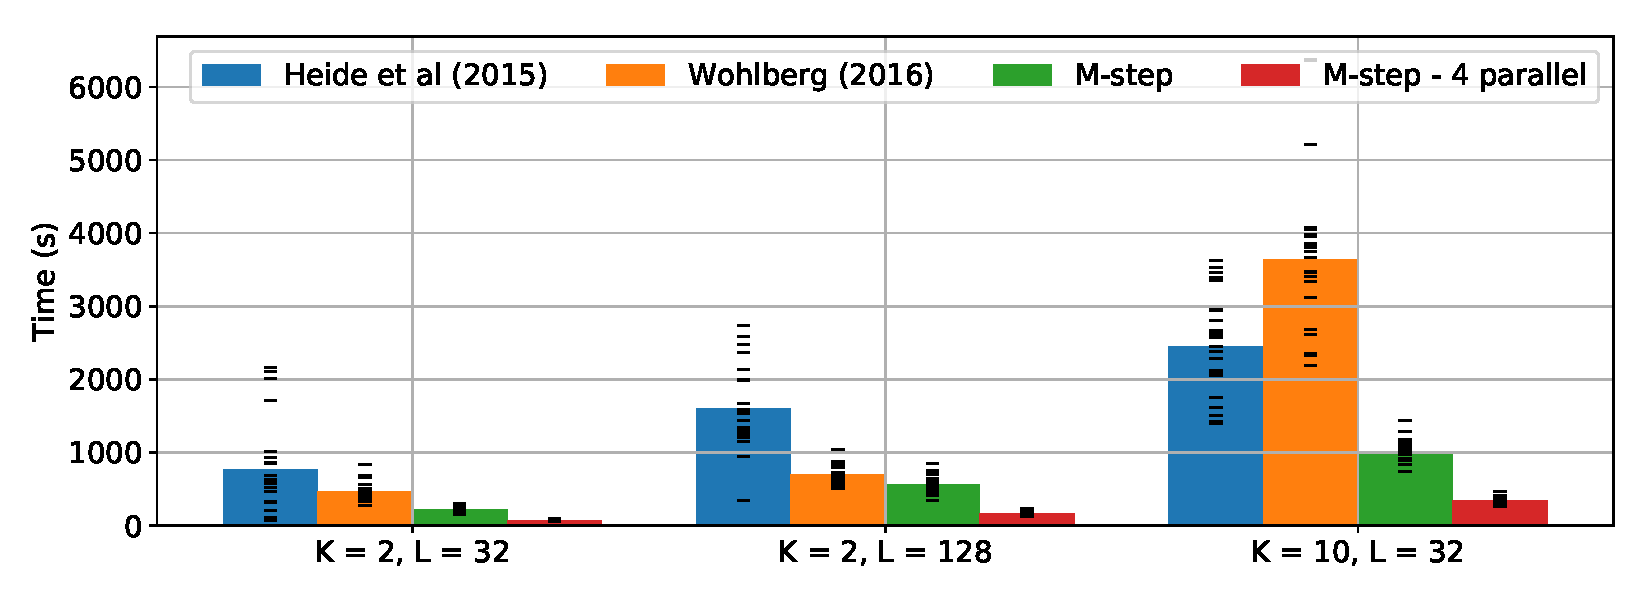
\includegraphics[width=\textwidth]{figures/bar_plot.pdf}}
    \caption[]{Comparison of state-of-the-art methods with our approach. (a)~Convergence plot with the objective function relative to the obtained minimum, as a function of computational time. (b)~Time taken to reach a relative precision of $10^{-2}$, for different settings of number of atoms $K$ and length of an atom $L$.  }
    \label{fig:sommaire:convergence}
\end{figure}

A \ac{CSC} model, as first introduced by \citep{grosse2012shift}, expresses the estimate signal $\hat{x}_n$ as a sum of convolution of atoms $d^k$ and their corresponding activations $z_n^k$:

\begin{align}
z_{n,t}^k \sim {\cal E}(\lambda),
\quad x_{n,t} | z, d \sim {\cal N}( \hat{x}_{n,t},1 ),
\quad \text{ where,}
\quad \hat{x}_n \triangleq \sum_{k=1}^{K}d^{k} * z_{n}^{k} \enspace .
\label{eqn:sommaire:csc_prob}
\end{align}

In the traditional model, the noise is assumed to be Gaussian distributed $\cal N(\cdot)$ and the activations are assumed sparse, drawn from an exponential distribution $\cal E(\cdot)$. The activations and atoms are estimated using an alternate minimization scheme. The model we introduce is a novel probabilistic \ac{CSC} model for learning shift-invariant atoms from unprocessed neural time series data containing potentially severe artifacts. Therefore, a Gaussian noise model is no longer sufficient. In the core of our model, which we call $\alpha$CSC, lies a family of heavy-tailed
distributions called $\alpha$-stable distributions. The parameter $\alpha$ controls how heavy-tailed the distribution is.

We develop a novel, computationally efficient \ac{MCEM} algorithm for inference. The maximization step boils down to a weighted
\ac{CSC} problem (Equation~\ref{eq:sommaire:problem_definition_z}), for which we develop a computationally efficient optimization algorithm.

\begin{align}
- & \max_{z, d} \sum_{n=1}^{N} \Big( \|\sqrt{w_{n}} \odot (x_{n} - \sum_{k=1}^{K}d^{k} * z_{n}^{k})\|_{2}^{2} + \lambda \sum_{k}{ \|{z}_{n}^{k} \|_1}\Big) \quad \text{ s.t.  } {z}_n^k \geq 0, \forall n,k\enspace .
\label{eq:sommaire:problem_definition_z}
\end{align} 

The weights $w_n$ in the maximization step are estimated in the expectation step using an \ac{MCMC} procedure. Indeed, the weights help us deal with the artifacts by suppressing them in the maximization step objective function.

\section*{Results}
\begin{figure}[htb]
    \centering
             \subfigure[LFP spike data from \cite{hitziger2017adaptive}]{
             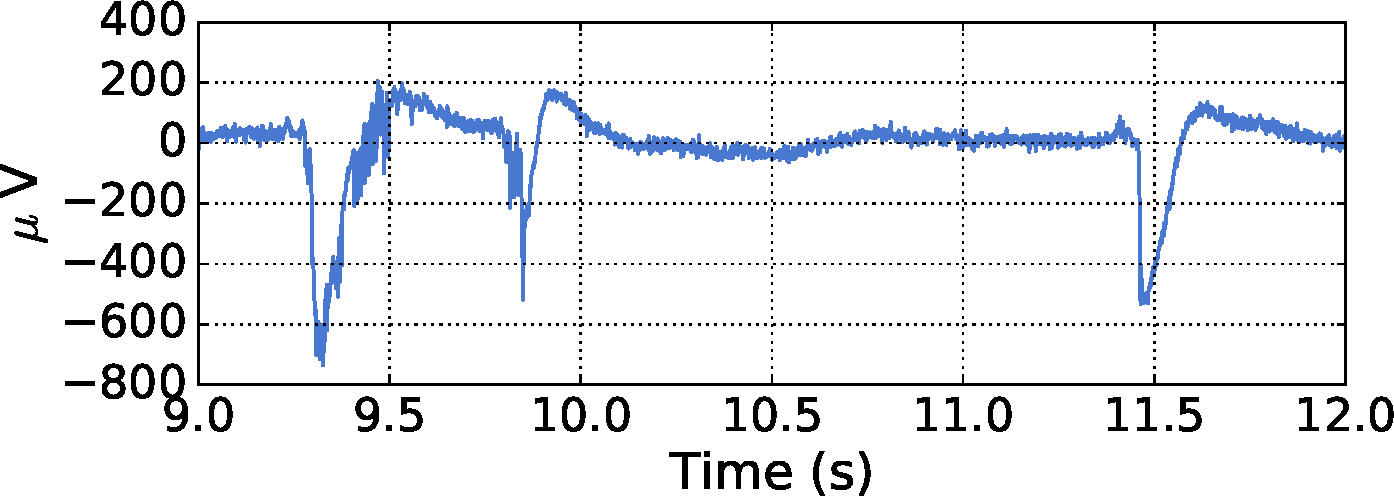
\includegraphics[height=4cm]{figures/spike_atomsa.pdf}
             } \\
             \subfigure[Estimated atoms]{
             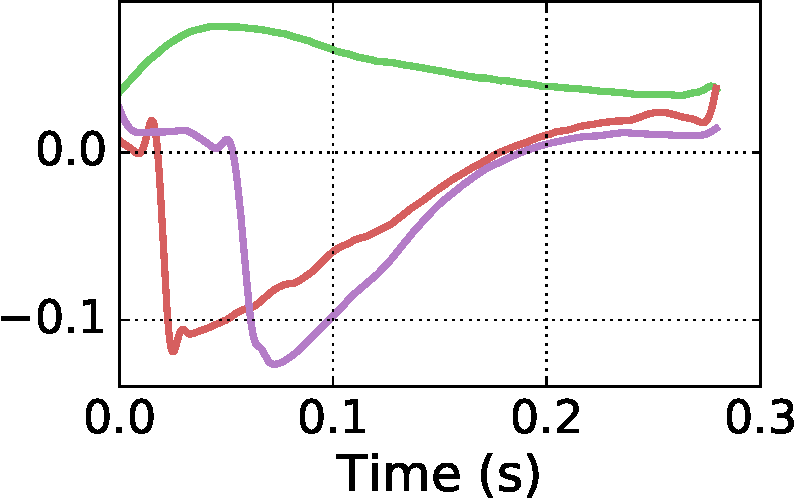
\includegraphics[height=4cm]{figures/spike_atomsb.pdf}
             }

            \caption[]{Atoms learnt by $\alpha$CSC on LFP data containing epileptiform spikes with $\alpha=2$.}
            \label{fig:sommaire:spikedata}
\end{figure}

In our work, we rigorously evaluate the computational efficiency of our algorithm against the competing benchmarks. Because the \ac{CSC} problem is non-convex, the optimization procedure involves nested loops and theoretical analysis often falls short in dealing with the complexity of non-convex functions. 
The optimization procedure is nested as the problem is convex when one of the variables is fixed: the atoms or the activations. The outer loop alternates between these two variables while the inner loop learns them when the other is fixed. The final result depends on the initialization, and therefore algorithms can be compared only if they are tested for many different random seeds and their results averaged. Our qualitative analysis also goes beyond the narrative of verifying the existence of known waveforms to uncovering more complex structures in the data.

Our results
show that the proposed algorithm achieves state-of-the-art convergence speeds (Figure~\ref{fig:sommaire:convergence}). Indeed, our algorithm uses quasi-Newton solvers which results in a faster convergence compared to ADMM-based methods~\citep{heide2015fast, wohlberg2016efficient}. Besides, $\alpha$CSC is
significantly more robust to artifacts when compared to three competing algorithms: it can extract
spike bursts (Figure~\ref{fig:sommaire:spikedata}), oscillations, and even reveal more subtle phenomena such as cross-frequency coupling
when applied to noisy neural time series.

\section*{Conclusion}

Methods research in neuroimaging is a marriage between computer science and neuroscience. It is a collaboration between two complementary disciplines -- the aim is to bring to the table computation tools which can help scientists make new discoveries. Certain aspects of this interdisciplinary subfield is of course to incrementally develop existing tools: for example, those that can help achieve a better prediction score, or a better localization accuracy in estimating neural sources. However, an orthogonal but equally important aspect of methods research is to develop tools which allow fundamentally new ways to interact with the data. This thesis is an attempt to advance this goal by developing tools for automated analysis in electrophysiology.

It has now become evident to us that in order to achieve the goal of reproducible research, large public datasets are the key and automated methods to analyze them are indispensable. While every neuroscientist's ambition is to generate new insights and push the frontiers of our knowledge of the brain, this is often not possible due to the weak effect sizes which cannot be uncovered in small datasets. When the null hypothesis cannot be rejected, it is a common practice to start fishing for significant results by testing multiple hypotheses and reporting the most favourable ones. This has resulted in a body of literature where a large fraction of the results lie on shaky grounds. 

In this thesis, we developed a new specification known as the \ac{BIDS}, which facilitates data sharing between neuroscientists by promoting common standards for storing measurement related metadata. We also provided an overview of the challenges in reproducible data analysis with respect to \ac{MEG}/\ac{EEG} data. As contributors to the MNE software package, we felt particularly well positioned to address  the software related challenges: complex pipelines, software versions, random initialization \emph{etc.,} and standardized recommendations for each stage of these pipelines. We did this by reanalyzing a group study on Faces dataset~\citep{wakeman2015multi}. To ensure reproducible results, the entire analysis was scripted and the plots generated automatically using the \code{sphinx\_gallery} package\footnote{https://sphinx-gallery.github.io}.

In order to even further push the goal of reproducibility via automation, we developed two new methods for analyzing electrophysiological data. The first method, called \emph{autoreject}, aims to streamline the removal of data segments containing artifacts which is a basic preprocessing step in almost every analysis chain. We develop an efficient method which uses a parameter search method known as Bayesian optimization. Our approach was able to facilitate re-analysis of the \ac{HCP} data for benchmarking. Our second method, known as \emph{alphacsc} enables mining neural time series for new oscillatory structures. Not only that, it is a tool to estimate more accurate waveform shapes than what is possible using traditional Fourier analysis. We demonstrated in our work that it was able to discover nested oscillations from the data.

These technologies can still be considered to be in their infancy in many respects. Just as source localization methods in \ac{MEG}/\ac{EEG} have evolved from dipole-based models to distributed methods to more sophisticated models implementing structured sparsity, these new methods are likely to undergo an evolutionary process of incremental improvements. If we consider the example of \ac{CSC}, our model based on alpha-stable distributions extended the computer vision models to be able to handle heavy-tailed distributions that is characteristic in neural data. Obviously, this is not the end of the road. Tuning hyperparameters in \ac{CSC} models is still notoriously difficult, but it is not impossible if there is an supervised task at the end of the pipeline. Multiscale dictionaries might be critical for brain signals considering that the oscillations can have varying support. As the problem is non-convex, smarter initialization strategies such as those based on \ac{MCMC} could lead to more accurate estimates~\citep{bachem2016fast}. It will also soon be necessary to build streaming \ac{CSC} algorithms based on stochastic approximations to deal with larger datasets.

Unlike computer vision or natural language processing, high-risk industries such as healthcare require transparent algorithms. It is no longer sufficient to be able to merely achieve higher prediction accuracy.
% In fact, a large fraction of neuroimaging data, even that which is available publicly, is unlabeled or at best weakly labeled.
In our work on \emph{autoreject} and \emph{alphacsc}, we leverage such public data to develop algorithms which are easy to interpret and diagnose. \emph{Autoreject} identifies the data segments to be removed based on a single parameter which is easy to understand and is automatically tuned. In the same way, \emph{alphacsc} mines the prototypical waveforms directly so as to replace indirect measures for unearthing phenomena of interest.

In this thesis, I outlined a strategy for reproducible research in the future: public datasets with large sample sizes and automation. However, the focus of some of my work was limited to automation on the scale of single subjects. Even though this does enable us to analyse large datasets, it can be sometimes limiting as it does not allow us to pool data across subjects so as to discover more subtle effects. As we enter an era of fast-paced science, such data-driven tools will become indispensable. While a lot of methods research has been focussed on improving the signal-to-noise ratio in each dataset, this may turn out to be not as important when dealing with larger datasets. Looking ahead, we will increasingly prefer large datasets which are not perfectly denoised rather than a smaller perfectly denoised dataset. New tools will need to be developed in order to enable clinicians to rapidly probe the brain so as to identify signals and structures of interest, quantify uncertainties along with the accuracy scores, perform quality control, and interactively visualize their data.
